% Author: Dr. Matthias Jung, DL9MJ
% Year: 2020
% TD431
\documentclass[convert = false, varwidth]{standalone}
\PassOptionsToPackage{locale=DE}{siunitx}
\PassOptionsToPackage{straightvoltages, europeanresistors, european inductor}{circuitikz}

\usepackage[locale=DE]{siunitx}
\usepackage{ifthen}
\usepackage{mathtools}
\usepackage{unicode-math}
\setmathfont{Libertinus Math}

\usepackage{circuitikz}
\makeatletter
\let\empty\relax
\makeatother
\usepackage{pgfplots}
\usepackage{pgfmath}
\usepackage{pgfplotstable}

\usepackage{etoolbox}
\usepackage{xcolor}
\usepackage{MnSymbol}

\usepackage{wasysym}
\usepackage{tikz-dimline}
\AtBeginDocument{\RenewCommandCopy\qty\SI} % Fix um qty doppeldefinition zu vermeiden 
\usepackage{tikz-3dplot}
%\usepackage{filecontents}% removed as obsolete

%TODO remove?
\usepackage{varwidth}
\usepackage{pgf-spectra}
\usepgfspectralibrary{pgfplots}

% TODO
% hier mal hart forciert, weil if ggf nicht geht?
% define colormap and check if cmyk is enforced
%\def\test#1{cmyk}
%\ifx\XC@tgt@mod\test
%	\pgfplotsset{colormap={slategraywhite}{cmyk=(0,0,0,.8) cmyk=(0,0,0,0)}}
%\else
	\pgfplotsset{colormap={slategraywhite}{rgb255=(50,50,50) rgb255=(255,255,255)}}
%\fi


\usetikzlibrary{math,perspective,intersections,arrows,arrows.meta,positioning,calc,shapes.symbols,decorations.pathmorphing,patterns,shapes.geometric,matrix,3d,backgrounds,babel,pgfplots.polar,decorations.pathreplacing,calligraphy,decorations.text,svg.path,optics}
\usepgfplotslibrary{fillbetween}
\pgfplotsset{compat=1.18}
\DeclareSIUnit{\baud}{Bd}

\sisetup{
    range-phrase=--,
    range-units=single
}

\usepackage[euler]{textgreek}

% Setze die Enden der optischen Pfeile etc. auf 60 grad:
\ctikzset{
	opto end arrow={Triangle[angle'=60]},
	tunable end arrow={Triangle}
}

% Grundsätzlich alle Pfeile als Triangle TODO, danach suchen und dann loeschen!
\tikzset{
    myarrow/.style={-Triangle}
}
\ctikzset{
    resistor=european,
    voltage=straight
}

\tikzstyle{digitalNumber}=[draw=DARCgray, fill=white, minimum width=0.5, minimum height=0.5, rounded corners=1, font=\bfseries]

% Gekritzelte Linie (Bild 315)
\pgfdeclaredecoration{penciline}{initial}{
	\state{initial}[width=+\pgfdecoratedinputsegmentremainingdistance,
	auto corner on length=1mm,]{
		\pgfpathcurveto%
		{% From
			\pgfqpoint{\pgfdecoratedinputsegmentremainingdistance}
			{\pgfdecorationsegmentamplitude}
		}
		{%  Control 1
			\pgfmathrand
			\pgfpointadd{\pgfqpoint{\pgfdecoratedinputsegmentremainingdistance}{0pt}}
			{\pgfqpoint{-\pgfdecorationsegmentaspect
					\pgfdecoratedinputsegmentremainingdistance}%
				{\pgfmathresult\pgfdecorationsegmentamplitude}
			}
		}
		{%TO
			\pgfpointadd{\pgfpointdecoratedinputsegmentlast}{\pgfpoint{1pt}{1pt}}
		}
	}
	\state{final}{}
}

% Bandplan bänder in Bild 750 und 749
\let\band\relax% conflict… requires cleanup … \providecommand? 
\newcommand{\band}[7]{%
    \draw[draw=red] (-5,#1) rectangle (5,#2);
    \draw ( 40,#1) node[right,rotate=0, text=red](){\footnotesize\textbf{\SI{#6}{#7}}};
    \draw ( 20,#1) node[rotate=0](){\footnotesize\SI{#3}{#5}};
    \draw (-20,#2) node[rotate=0](){\footnotesize\SI{#4}{#5}};
}

\let\bandB\relax% conflict… requires cleanup … \providecommand? 
\newcommand{\bandB}[7]{%
    \draw[draw=red] (-5,#1) rectangle (5,#2);
    \draw ( 40,#1) node[right,rotate=0, text=red](){\footnotesize\textbf{\SI{#6}{#7}}};
    \draw ( 20,#1) node[rotate=0,above](){\footnotesize\SI{#3}{#5}};
    \draw (-20,#2) node[rotate=0,above](){\footnotesize\SI{#4}{#5}};
}

\newcommand{\bandC}[7]{%
    \draw[draw=red] (#1,-5) rectangle (#2,5);
    \draw (#1, 65.0) node[rotate=-90, text=red](){\footnotesize\textbf{\SI{#6}{#7}}};
    \draw (#1, 27.5) node[rotate=-90](){\footnotesize\SI{#3}{#5}};
    \draw (#2,-27.5) node[rotate=-90](){\footnotesize\SI{#4}{#5}};
}

\newcommand{\bandD}[5]{%
    \draw[draw=red] (#1,-5) rectangle (#2,5);
    \draw (#1+50000000, 27.5) node[rotate=-90](){\footnotesize\SI{#3}{#5}};
    \draw (#2+50000000,-27.5) node[rotate=-90](){\footnotesize\SI{#4}{#5}};
}

% Symbol für das Gleichstrom
\newcommand{\textdirectcurrent}{%
  \settowidth{\dimen0}{$=$}%
  \vbox to .85ex {\offinterlineskip
    \hbox to \dimen0{\leaders\hrule\hfill}
    \vskip.35ex
    \hbox to \dimen0{%
      \leaders\hrule\hskip.2\dimen0\hfill
      \leaders\hrule\hskip.2\dimen0\hfill
      \leaders\hrule\hskip.2\dimen0
    }
    \vfill
  }%
}
\newcommand{\mathdirectcurrent}{\mathrel{\textdirectcurrent}}

% Zum Messen von Abständen
\makeatletter
\newcommand{\Distance}[3]{% from https://tex.stackexchange.com/q/56353/121799
	\tikz@scan@one@point\pgfutil@firstofone($#1-#2$)\relax  
	\pgfmathsetmacro{#3}{round(0.99626*veclen(\the\pgf@x,\the\pgf@y)/0.0283465)/1000}
}
\makeatother

% Bemaßung zeichnen:
\NewDocumentCommand\DARCmeasure{O{black} O{middle} m m m m m}{% 1:[color], 2:[top], 3:start, 4:end, 5:shift, 6:rotate, 7:text
    \path($(#3)+(#5)$) coordinate(start);
    \path($(#4)+(#5)$) coordinate(end);
    \ifthenelse{\equal{#2}{top}}{
        \draw ($(start)!0.5!(end)$) coordinate(middle);
        \node[rotate=#6, anchor=south] (text) at (middle) {\textcolor{#1}{#7}};
        \draw[draw=#1, |Triangle-] (start) -- (middle);
        \draw[draw=#1, |Triangle-] (end) -- (middle);
    }{
        \node[rotate=#6] (text) at ($(start)!0.5!(end)$) {\textcolor{#1}{#7}};
        \draw[draw=#1, |Triangle-] (start) -- (text.west);
        \draw[draw=#1, |Triangle-] (end) -- (text.east);
    }
}

% Magic von Marei zur Skalierung der Bilder
\makeatletter
\ExplSyntaxOn
\box_new:N \l_ptxcd_image_box

\cs_if_exist:NF \if@DARCinQuestion {\newif\if@DARCinQuestion}

\fp_if_exist:NF \l_ptxcd_tmp_fp {\fp_new:N \l_ptxcd_tmp_fp}
\fp_set:Nn \l_ptxcd_tmp_fp  {1}

\int_new:N \g_DARC_image_fail_int
\seq_new:N \g__DARC_image_fail_seq
\dim_new:N \l__DARC_image_width_dim
\box_new:N \l_ptxcd_image_orig_box

\newcommand*{\getDarcImageFactor}{\fp_use:N  \l_ptxcd_tmp_fp}



\NewDocumentCommand{\DARCimageOnly}{smm}{
	\setmathfont{Libertinus Math}
	 \ptxcd_image_autoscale_setup:nnn {#1} {#2} {#3}
		\usepackage{geometry}
        \usepackage{}
	\geometry{paperwidth=\box_wd:N  \l_ptxcd_image_box, paperheight=\box_ht_plus_dp:N  \l_ptxcd_image_box,margin=0pt}
	\pagestyle{empty}
	\setlength{\topskip}{0pt}% necessary because otherwhise \topskip could exceed \paperheight
	\begin{document}
		\box_use:N \l_ptxcd_image_box
	\end{document}
}

\seq_new:N  \g__ptxcd_image_size_seq
\prop_new:N \g__ptxcd_image_size_cache_prop
\bool_new:N \l__ptxcd_disable_autoscale_bool
\newcommand*{\disableDARCautoscale}{\bool_set_true:N  \l__ptxcd_disable_autoscale_bool}

\cs_new:Nn \ptxcd_image_autoscale_setup:nnn {
	\prop_if_in:NnTF \g__ptxcd_image_size_cache_prop {#2} {
			\fp_set:Nn \l_ptxcd_tmp_fp {\prop_item:Nn \g__ptxcd_image_size_cache_prop {#2}}
			\hbox_gset:Nn \l_ptxcd_image_box {
				\tikzset{x=\fp_use:N \l_ptxcd_tmp_fp cm,y=\fp_use:N \l_ptxcd_tmp_fp cm}
				\file_if_exist_input:n {img/#2}%
				\ifvmode\else\unskip\fi
			}
		\seq_gput_right:Nx \g__ptxcd_image_size_seq {#2=\prop_item:Nn \g__ptxcd_image_size_cache_prop {#2}}
	} {
		\hbox_gset:Nn \l_ptxcd_image_orig_box {
			\file_if_exist_input:n {img/#3}%
			\ifvmode\else\unskip\fi%
		}
		\bool_if:NT \l__ptxcd_disable_autoscale_bool \use_iii:nnnn
		\IfBooleanTF{#1}{
			\box_gset_eq:NN \l_ptxcd_image_box \l_ptxcd_image_orig_box
		} {
			\dim_compare:nNnTF {\box_wd:N \l_ptxcd_image_orig_box} = {\c_zero_dim} {
				\fp_set:Nn  \l_ptxcd_tmp_fp {1}
			} {
				\if@DARCinQuestion
					\dim_compare:nTF {#2 =\linewidth} {
						\dim_set:Nn  \l__DARC_image_width_dim {\columnwidth}
					} {
						\dim_set:Nn  \l__DARC_image_width_dim {#2}
					}
				\else
					\dim_set:Nn  \l__DARC_image_width_dim {#2}
				\fi
				\fp_set:Nn \l_ptxcd_tmp_fp {\dim_to_decimal_in_unit:nn {\l__DARC_image_width_dim} {\box_wd:N \l_ptxcd_image_orig_box}}
				\hbox_gset:Nn \l_ptxcd_image_box {
					\tikzset{x=\fp_use:N \l_ptxcd_tmp_fp cm,y=\fp_use:N \l_ptxcd_tmp_fp cm}
					\file_if_exist_input:n {img/#3}%
					\ifvmode\else\unskip\fi
				}
				\bool_lazy_and:nnT
					{ \dim_compare_p:nNn {\box_wd:N \l_ptxcd_image_box} < {\l__DARC_image_width_dim  -1em} }
					{ ! \dim_compare_p:nNn {\box_wd:N \l_ptxcd_image_box} = {\box_wd:N \l_ptxcd_image_orig_box}}
				{
					\fp_set:Nn \l_ptxcd_tmp_fp { 1 + \dim_to_decimal_in_unit:nn {\l__DARC_image_width_dim- \box_wd:N \l_ptxcd_image_orig_box} {\box_wd:N \l_ptxcd_image_box - \box_wd:N \l_ptxcd_image_orig_box} * (\l_ptxcd_tmp_fp  -1)}
					\hbox_gset:Nn \l_ptxcd_image_box {
						\tikzset{x=\fp_use:N \l_ptxcd_tmp_fp cm,y=\fp_use:N \l_ptxcd_tmp_fp cm}
						\file_if_exist_input:n {img/#3}%
						\ifvmode\else\unskip\fi
					}
				}
				\dim_compare:nNnTF  {\box_wd:N \l_ptxcd_image_box} = {\box_wd:N \l_ptxcd_image_orig_box} {
					\seq_gput_right:Nx \g__ptxcd_image_size_seq {#3=1}
				}{
					\seq_gput_right:Nx \g__ptxcd_image_size_seq {#3=\fp_use:N \l_ptxcd_tmp_fp}
				}
			}
		}
	}
}

\newcommand*{\DARCimageCache}[1]{
	\prop_gset_from_keyval:Nn \g__ptxcd_image_size_cache_prop {#1}
}

\hook_gput_code:nnn {enddocument/afterlastpage}{write-DARCimage-size-cache}{
	\iow_now:Ne \@auxout {
		\exp_not:N \DARCimageCache{
			\seq_use:Nn  \g__ptxcd_image_size_seq {,}
		}
	}
}

\NewDocumentCommand{\DARCimage}{sO{Bild~zur~Prüfungsfrage~\l_ptxcd_question_tl}mm}{
	\par\smallskip
	\begingroup
		\ptxcd_image_autoscale_setup:nnn {#1} {#3} {#4}
		\dim_compare:nNnTF {\box_wd:N \l_ptxcd_image_box} > {\linewidth}
		{
			\makebox[\linewidth][r]{\box_use:N \l_ptxcd_image_box}
		} {
			\makebox[\linewidth][c]{\box_use:N \l_ptxcd_image_box}
		}
	\endgroup
}
\ExplSyntaxOff
\makeatother

% Neue TL, wird bald in einem zukünftigen circuittikz sein: 
% https://github.com/circuitikz/circuitikz/issues/694
\makeatletter
\newif\ifpgf@circ@bare@tline
\ctikzset{bipoles/tline/bare/.is if=pgf@circ@bare@tline}
\pgfcircdeclarebipolescaled{RF}
{
\savedmacro{\recessright}{\edef\recessright{\ifpgf@circ@bare@tline -0.4\else 0.0\fi}}
\anchor{center right}{\northeast \advance\pgf@x by -0.4\pgf@y\pgf@y=0pt}
\anchor{top right}{\northeast \advance\pgf@x by -0.4\pgf@y}
\anchor{bottom right}{\northeast \advance\pgf@x by -0.4\pgf@y\pgf@y=-\pgf@y}
\anchor{center left}{\northeast \advance\pgf@x by -0.4\pgf@y\pgf@x=-\pgf@x\pgf@y=0pt}
\anchor{top left}{\northeast \advance\pgf@x by -0.4\pgf@y\pgf@x=-\pgf@x}
\anchor{bottom left}{\northeast \advance\pgf@x by -0.4\pgf@y\pgf@x=-\pgf@x\pgf@y=-\pgf@y}
\anchor{right}{\northeast \advance\pgf@x by \recessright\pgf@y\pgf@y=0pt}
}
{\ctikzvalof{bipoles/tline/height}}
{tline}
{\ctikzvalof{bipoles/tline/height}}
{\ctikzvalof{bipoles/tline/width}}
{
\pgf@circ@res@step=.4\pgf@circ@res@up % the size of the ellipsis is proportional to the height
\pgfscope
\pgf@circ@setlinewidth{bipoles}{\pgfstartlinewidth}
\pgfpathmoveto{\pgfpoint{\pgf@circ@res@right-\pgf@circ@res@step}{\pgf@circ@res@up}}
\pgfpathlineto{\pgfpoint{\pgf@circ@res@left+\pgf@circ@res@step}{\pgf@circ@res@up}}
\pgfpatharc{-90}{90}{-\pgf@circ@res@step and -\pgf@circ@res@up}
\pgfpathlineto{\pgfpoint{\pgf@circ@res@right-\pgf@circ@res@step}{\pgf@circ@res@down}}
\pgfpatharc{-90}{90}{\pgf@circ@res@step and \pgf@circ@res@up}
\pgf@circ@draworfill
\pgfpathmoveto{\pgfpoint{\pgf@circ@res@right-\pgf@circ@res@step}{\pgf@circ@res@up}}
\pgfpatharc{-90}{90}{-\pgf@circ@res@step and -\pgf@circ@res@up}
\pgfusepath{stroke}
\endpgfscope
\ifpgf@circ@bare@tline\else
\pgfsetlinewidth{\pgfstartlinewidth}
\pgfpathmoveto{\pgfpoint{\pgf@circ@res@right-\pgf@circ@res@step}{0pt}}
\pgfpathlineto{\pgfpoint{\pgf@circ@res@right}{0pt}}
\pgfusepath{stroke}
\fi
}
\makeatother

% Neues mikrofon, wird irgendwann teil von circuit tikzi und kann dann hier
% gelöscht werden: https://github.com/circuitikz/circuitikz/issues/689
% <
\makeatletter
\ctikzset{bipoles/tlmic/height/.initial=.5}
\ctikzset{bipoles/tlmic/depth/.initial=.5}
\ctikzset{bipoles/tlmic/width/.initial=.5}%
\pgfcircdeclarebipolescaled{misc}
{}
{\ctikzvalof{bipoles/tlmic/depth}}
{tlmic}
{\ctikzvalof{bipoles/tlmic/height}}
{\ctikzvalof{bipoles/tlmic/width}}{

    \pgf@circ@setlinewidth{bipoles}{\pgfstartlinewidth}
    \pgfpathcircle{\pgfpoint{0pt}{0pt}}{\pgf@circ@res@up}
    \pgf@circ@draworfill
    \pgfpathmoveto{\pgfpoint{\pgf@circ@res@left}{\pgf@circ@res@up}}
    \pgfpathlineto{\pgfpoint{\pgf@circ@res@right}{\pgf@circ@res@up}}
    \pgfusepath{draw}
}
\pgfcirc@activate@bipole@simple{l}{tlmic}

\makeatother
% />

% Power Plug
\makeatletter
\ctikzset{bipoles/plug/height/.initial=.5}
\ctikzset{bipoles/plug/width/.initial=.5}%
\pgfcircdeclarebipolescaled{misc}
{}
{\ctikzvalof{bipoles/plug/height}}
{plug}
{\ctikzvalof{bipoles/plug/height}}
{\ctikzvalof{bipoles/plug/width}}{

    %\pgf@circ@setlinewidth{bipoles}{\pgfstartlinewidth}
    \pgfpathcircle{\pgfpoint{0pt}{0pt}}{\pgf@circ@res@up}
	\pgfusepath{fill}
    %\pgfpathmoveto{\pgfpoint{\pgf@circ@res@left}{\pgf@circ@res@up}}
    %\pgfpathlineto{\pgfpoint{\pgf@circ@res@right}{\pgf@circ@res@up}}
    %\pgfusepath{draw}
	% Plus:
	\color{black} 
	\pgfsetstrokecolor{black} 
	\pgfpathrectangle{\pgfpoint{0.0\pgf@circ@res@step}{-0.1\pgf@circ@res@step}}{\pgfpoint{-0.2\pgf@circ@res@step}{+0.1\pgf@circ@res@step}}%
	\pgfusepath{fill}
}
\pgfcirc@activate@bipole@simple{l}{plug}
\makeatother

%% bgenerator und bgeneratorshape block
% Eine submission nach circuittikz wurde durchgeführt: 
% https://github.com/circuitikz/circuitikz/pull/693
% <
\makeatletter
%
\def\pgfcirc@twoport@draw@narrowsine#1{% #1 -> y shift
    \pgfscope
        \pgfsetlinewidth{\pgfstartlinewidth}
        \pgftransformyshift{#1\pgf@circ@res@step}
        \pgfpathmoveto{\pgfpoint{.125\pgf@circ@res@step}{0\pgf@circ@res@step}}
        \pgfpathsine{\pgfpoint{.125\pgf@circ@res@step}{.125\pgf@circ@res@step}}
        \pgfpathcosine{\pgfpoint{.125\pgf@circ@res@step}{-.125\pgf@circ@res@step}}
        \pgfpathsine{\pgfpoint{.125\pgf@circ@res@step}{-.125\pgf@circ@res@step}}
        \pgfpathcosine{\pgfpoint{.125\pgf@circ@res@step}{.125\pgf@circ@res@step}}
        \pgfusepath{draw}
    \endpgfscope
}
%
\ctikzset{bipoles/bgenerator/width/.initial=.7}
\pgfcirc@define@twoports{blocks}
{}
{\ctikzvalof{bipoles/bgenerator/width}}
{bgenerator}
{\ctikzvalof{bipoles/bgenerator/width}}
{\ctikzvalof{bipoles/bgenerator/width}}
{
    \pgfcirc@twoport@draw@narrowsine{0.25}{0}
    \pgfcirc@twoport@draw@narrowsine{0.0}{0}
    \pgfcirc@twoport@draw@narrowsine{-0.25}{0}
    \pgftext[x=0.45\pgf@circ@res@left]{\ctikzvalof{bipoles/twoport/text}}
}
\pgfcirc@activate@bipole@simple{l}{bgenerator}
\makeatother
%>

%Q-Generator TODO: Update pull request
\makeatletter
%
\ctikzset{bipoles/qgenerator/width/.initial=.7}
\pgfcirc@define@twoports{blocks}
{}
{\ctikzvalof{bipoles/qgenerator/width}}
{qgenerator}
{\ctikzvalof{bipoles/qgenerator/width}}
{\ctikzvalof{bipoles/qgenerator/width}}
{
    \pgfcirc@twoport@draw@narrowsine{0.45}{0}
    \pgfcirc@twoport@draw@narrowsine{0.20}{0}
    \pgfcirc@twoport@draw@narrowsine{-0.05}{0}
    \pgftext[x=0.45\pgf@circ@res@left,y=0.25\pgf@circ@res@up]{\ctikzvalof{bipoles/twoport/text}}
	\pgfpathmoveto{\pgfpoint{-0.7\pgf@circ@res@step}{-0.35\pgf@circ@res@step}} 
	\pgfpathlineto{\pgfpoint{ 0.7\pgf@circ@res@step}{-0.35\pgf@circ@res@step}} 
    \pgfusepath{draw}
	\pgfpathrectangle{\pgfpoint{-0.7\pgf@circ@res@step}{-0.7\pgf@circ@res@step}}{\pgfpoint{1.4\pgf@circ@res@step}{0.2\pgf@circ@res@step}} 
    \pgfusepath{draw}
	\pgfpathmoveto{\pgfpoint{-0.7\pgf@circ@res@step}{-0.85\pgf@circ@res@step}} 
	\pgfpathlineto{\pgfpoint{ 0.7\pgf@circ@res@step}{-0.85\pgf@circ@res@step}} 
    \pgfusepath{draw}
}
\pgfcirc@activate@bipole@simple{l}{qgenerator}
\makeatother

%Clock-Generator TODO: Add to pull request
\makeatletter
%
\ctikzset{bipoles/cgenerator/width/.initial=.7}
\pgfcirc@define@twoports{blocks}
{}
{\ctikzvalof{bipoles/cgenerator/width}}
{cgenerator}
{\ctikzvalof{bipoles/cgenerator/width}}
{\ctikzvalof{bipoles/cgenerator/width}}
{
	\pgfpathmoveto{\pgfpoint{-0.70\pgf@circ@res@step}{-0.35\pgf@circ@res@step}} 
	\pgfpathlineto{\pgfpoint{-0.42\pgf@circ@res@step}{-0.35\pgf@circ@res@step}} 
	\pgfpathlineto{\pgfpoint{-0.42\pgf@circ@res@step}{+0.35\pgf@circ@res@step}} 
	\pgfpathlineto{\pgfpoint{-0.14\pgf@circ@res@step}{+0.35\pgf@circ@res@step}} 
	\pgfpathlineto{\pgfpoint{-0.14\pgf@circ@res@step}{-0.35\pgf@circ@res@step}} 
	\pgfpathlineto{\pgfpoint{+0.14\pgf@circ@res@step}{-0.35\pgf@circ@res@step}} 
	\pgfpathlineto{\pgfpoint{+0.14\pgf@circ@res@step}{+0.35\pgf@circ@res@step}} 
	\pgfpathlineto{\pgfpoint{+0.42\pgf@circ@res@step}{+0.35\pgf@circ@res@step}} 
	\pgfpathlineto{\pgfpoint{+0.42\pgf@circ@res@step}{-0.35\pgf@circ@res@step}} 
	\pgfpathlineto{\pgfpoint{+0.70\pgf@circ@res@step}{-0.35\pgf@circ@res@step}} 
    \pgfusepath{draw}
}
\pgfcirc@activate@bipole@simple{l}{cgenerator}
\makeatother

%Sine Table: TODO in pullrequest packen
\makeatletter
%
\ctikzset{bipoles/sinetable/width/.initial=.7}
\pgfcirc@define@twoports{blocks}
{}
{\ctikzvalof{bipoles/sinetable/width}}
{sinetable}
{\ctikzvalof{bipoles/sinetable/width}}
{\ctikzvalof{bipoles/sinetable/width}}
{
    \pgfcirc@twoport@draw@sine{0.0}{0}
    \pgfcirc@set@arrows{tunable}{}{latex}
	\pgfpathmoveto{\pgfpoint{-0.70\pgf@circ@res@step}{-0.70\pgf@circ@res@step}} 
	\pgfpathlineto{\pgfpoint{+0.70\pgf@circ@res@step}{-0.70\pgf@circ@res@step}} 
    \pgfusepath{draw}
	\pgfpathmoveto{\pgfpoint{-0.70\pgf@circ@res@step}{-0.70\pgf@circ@res@step}} 
	\pgfpathlineto{\pgfpoint{-0.70\pgf@circ@res@step}{+0.70\pgf@circ@res@step}} 
    \pgfusepath{draw}
}
\pgfcirc@activate@bipole@simple{l}{sinetable}
\makeatother

%Sine Table: TODO in pullrequest packen
\makeatletter
%
\ctikzset{bipoles/register/width/.initial=.7}
\pgfcirc@define@twoports{blocks}
{
	\savedanchor\northwest{
		\pgfmathsetlength{\pgf@circ@scaled@Rlen}{\ctikzvalof{\ctikzclass/scale}\pgf@circ@Rlen}
		\pgf@y=\ctikzvalof{bipoles/twoport/width}\pgf@circ@scaled@Rlen
		\pgf@y=.5\pgf@y
		\pgf@x=-\ctikzvalof{bipoles/twoport/width}\pgf@circ@scaled@Rlen
		\pgf@x=.5\pgf@x
	}
	\anchor{clk}{\northwest\pgf@y=0.5\pgf@y}
}
{\ctikzvalof{bipoles/register/width}}
{register}
{\ctikzvalof{bipoles/register/width}}
{\ctikzvalof{bipoles/register/width}}
{
	\pgfpathmoveto{\pgfpoint{-1.00\pgf@circ@res@step}{+0.70\pgf@circ@res@step}} 
	\pgfpathlineto{\pgfpoint{-0.60\pgf@circ@res@step}{+0.50\pgf@circ@res@step}} 
	\pgfpathlineto{\pgfpoint{-1.00\pgf@circ@res@step}{+0.30\pgf@circ@res@step}} 
    \pgfusepath{draw}
}
\pgfcirc@activate@bipole@simple{l}{register}
\makeatother

%% Bias-T
% TODO, add to pull request
\makeatletter
\ctikzset{bipoles/biast/width/.initial=.7}
\pgfcirc@define@twoports{blocks}
{}
{\ctikzvalof{bipoles/biast/width}}
{biast}
{\ctikzvalof{bipoles/biast/width}}
{\ctikzvalof{bipoles/biast/width}}
{
	\pgfpathmoveto{\pgfpoint{-0.80\pgf@circ@res@step}{-0.50\pgf@circ@res@step}} % Line to Plate 1
	\pgfpathlineto{\pgfpoint{-0.50\pgf@circ@res@step}{-0.50\pgf@circ@res@step}} 
	\pgfpathmoveto{\pgfpoint{-0.50\pgf@circ@res@step}{-0.50\pgf@circ@res@step}} % Plate 1
	\pgfpathlineto{\pgfpoint{-0.50\pgf@circ@res@step}{-0.20\pgf@circ@res@step}} 
	\pgfpathmoveto{\pgfpoint{-0.50\pgf@circ@res@step}{-0.50\pgf@circ@res@step}} 
	\pgfpathlineto{\pgfpoint{-0.50\pgf@circ@res@step}{-0.80\pgf@circ@res@step}} 
	\pgfpathmoveto{\pgfpoint{-0.30\pgf@circ@res@step}{-0.50\pgf@circ@res@step}} % Plate 1
	\pgfpathlineto{\pgfpoint{-0.30\pgf@circ@res@step}{-0.20\pgf@circ@res@step}} 
	\pgfpathmoveto{\pgfpoint{-0.30\pgf@circ@res@step}{-0.50\pgf@circ@res@step}} 
	\pgfpathlineto{\pgfpoint{-0.30\pgf@circ@res@step}{-0.80\pgf@circ@res@step}}
	\pgfpathmoveto{\pgfpoint{-0.30\pgf@circ@res@step}{-0.50\pgf@circ@res@step}} % Line to Center
	\pgfpathlineto{\pgfpoint{ 0.00\pgf@circ@res@step}{-0.50\pgf@circ@res@step}} 
    \pgfusepath{draw}
    \pgfpathcircle{\pgfpoint{ 0.00\pgf@circ@res@step}{-0.50\pgf@circ@res@step}}{0.075\pgf@circ@res@step}
    \pgfusepath{fill}
	\pgfpathmoveto{\pgfpoint{ 0.00\pgf@circ@res@step}{-0.50\pgf@circ@res@step}} % Line to Right
	\pgfpathlineto{\pgfpoint{ 0.80\pgf@circ@res@step}{-0.50\pgf@circ@res@step}} 
    \pgfusepath{draw}
	\pgfpathmoveto{\pgfpoint{ 0.00\pgf@circ@res@step}{-0.50\pgf@circ@res@step}} % Line to Coils
	\pgfpathlineto{\pgfpoint{ 0.00\pgf@circ@res@step}{-0.20\pgf@circ@res@step}} 
    \pgfusepath{draw}
	\pgfpathmoveto{\pgfpoint{ 0.00\pgf@circ@res@step}{-0.20\pgf@circ@res@step}} % Arc1
	\pgfpatharc{-90}{90}{0.09\pgf@circ@res@step}
	\pgfpathmoveto{\pgfpoint{ 0.00\pgf@circ@res@step}{-0.02\pgf@circ@res@step}} % Arc2
	\pgfpatharc{-90}{90}{0.09\pgf@circ@res@step}
	\pgfpathmoveto{\pgfpoint{ 0.00\pgf@circ@res@step}{+0.16\pgf@circ@res@step}} % Arc3
	\pgfpatharc{-90}{90}{0.09\pgf@circ@res@step}
	\pgfpathmoveto{\pgfpoint{ 0.00\pgf@circ@res@step}{+0.36\pgf@circ@res@step}} % Arc4
	\pgfpatharc{-90}{90}{0.09\pgf@circ@res@step}
	\pgfusepath{draw}
	\pgfpathmoveto{\pgfpoint{ 0.00\pgf@circ@res@step}{+0.52\pgf@circ@res@step}} % Line to Coils
	\pgfpathlineto{\pgfpoint{ 0.00\pgf@circ@res@step}{+0.80\pgf@circ@res@step}} 
	\pgfusepath{draw}
}
\pgfcirc@activate@bipole@simple{l}{biast}
\makeatother

%% variable allpass filter
% Eine submission nach circuittikz wurde durchgeführt: 
% https://github.com/circuitikz/circuitikz/pull/693
\makeatletter
\ctikzset{bipoles/vallpass/width/.initial=.7}
\pgfcirc@define@twoports{blocks}
{}
{\ctikzvalof{bipoles/vallpass/width}}
{vallpass}
{\ctikzvalof{bipoles/vallpass/width}}
{\ctikzvalof{bipoles/vallpass/width}}
{
    \pgfcirc@twoport@draw@sine{0.5}{0}
    \pgfcirc@twoport@draw@sine{0.0}{0}
    \pgfcirc@twoport@draw@sine{-0.5}{0}
    \pgfcirc@set@arrows{tunable}{}{latex}
    \pgfpathmoveto{\pgfpoint{0.7\pgf@circ@res@left}{0.5\pgf@circ@res@down}}
    \pgfpathlineto{\pgfpoint{0.7\pgf@circ@res@right}{0.8\pgf@circ@res@up}}
    \pgfusepath{draw}
}
\pgfcirc@activate@bipole@simple{l}{vallpass}
\makeatother

%% bgenerator und bgeneratorshape block
% <
\makeatletter
%
\ctikzset{bipoles/ngenerator/width/.initial=.7}
\pgfcirc@define@twoports{blocks}
{}
{\ctikzvalof{bipoles/ngenerator/width}}
{ngenerator}
{\ctikzvalof{bipoles/ngenerator/width}}
{\ctikzvalof{bipoles/ngenerator/width}}
{
    \pgfcirc@twoport@draw@sine{0.5}{0}
    \pgftext[y=-0.35\pgf@circ@res@up]{\ctikzvalof{bipoles/twoport/text}}
}
\pgfcirc@activate@bipole@simple{l}{ngenerator}
\makeatother
%>

% Camera
% has to be commited to PR
\makeatletter
\ctikzset{bipoles/camera/height/.initial=1.2}
\ctikzset{bipoles/camera/depth/.initial=.3}
\ctikzset{bipoles/camera/width/.initial=.4}
\pgfcircdeclarebipolescaled{misc}
{}
{\ctikzvalof{bipoles/camera/depth}}
{camera}
{\ctikzvalof{bipoles/camera/height}}
{\ctikzvalof{bipoles/camera/width}}{
    \pgfpathrectanglecorners{\pgfpoint{\pgf@circ@res@left}{.7\pgf@circ@res@up}}
    {\pgfpoint{\pgf@circ@res@right}{\pgf@circ@res@down}}
    \pgfpathmoveto{\pgfpoint{0.5\pgf@circ@res@left}{.7\pgf@circ@res@up}}
    \pgfpathlineto{\pgfpoint{0.8\pgf@circ@res@left}{\pgf@circ@res@up}}
    \pgfpathlineto{\pgfpoint{0.8\pgf@circ@res@right}{\pgf@circ@res@up}}
    \pgfpathlineto{\pgfpoint{0.5\pgf@circ@res@right}{.7\pgf@circ@res@up}}
    \pgfpathclose
    \pgf@circ@setlinewidth{bipoles}{\pgfstartlinewidth}
    \pgf@circ@draworfill
}
\pgfcirc@activate@bipole@simple{l}{camera}

\makeatother

% TRX
% has to be commited to PR
\makeatletter
\ctikzset{bipoles/trx/width/.initial=1}
\ctikzset{bipoles/trx/height/.initial=.4}
\pgfcirc@define@twoports{blocks}
{
	\anchor{plus}{\northeast \advance\pgf@y by -0.2\pgf@x\pgf@x=-\pgf@x}
	\anchor{minus}{\northeast \advance\pgf@y by -0.2\pgf@x\pgf@x=-\pgf@x\pgf@y=-\pgf@y}
}
{\ctikzvalof{bipoles/trx/height}}
{trx}
{\ctikzvalof{bipoles/trx/height}}
{\ctikzvalof{bipoles/trx/width}}
{
	% VFO-Rad:
	\pgfpathcircle{\pgfpoint{0.60\pgf@circ@res@step}{0.00\pgf@circ@res@step}}{0.25\pgf@circ@res@step}
	\pgfpathcircle{\pgfpoint{0.68\pgf@circ@res@step}{0.10\pgf@circ@res@step}}{0.06\pgf@circ@res@step}
	% Lautstärke und Rauschsperre:
	\pgfpathcircle{\pgfpoint{-0.8\pgf@circ@res@step}{+0.15\pgf@circ@res@step}}{0.1\pgf@circ@res@step}
	\pgfpathcircle{\pgfpoint{-0.8\pgf@circ@res@step}{-0.15\pgf@circ@res@step}}{0.1\pgf@circ@res@step}
	% Bildschirm:
	\pgfpathrectangle{\pgfpoint{-0.55\pgf@circ@res@step}{-0.25\pgf@circ@res@step}}{\pgfpoint{+0.75\pgf@circ@res@step}{+0.5\pgf@circ@res@step}}%
    \pgfusepath{draw}
}
\pgfcirc@activate@bipole@simple{l}{trx}
\makeatother

% SWR
% has to be commited to PR
\makeatletter
\ctikzset{bipoles/swr/width/.initial=0.6}
\ctikzset{bipoles/swr/height/.initial=.4}
\pgfcirc@define@twoports{blocks}
{}
{\ctikzvalof{bipoles/swr/height}}
{swr}
{\ctikzvalof{bipoles/swr/height}}
{\ctikzvalof{bipoles/swr/width}}
{
	% Bildschirm:
	\pgfpathrectangle{\pgfpoint{-0.6\pgf@circ@res@step}{-0.4\pgf@circ@res@step}}{\pgfpoint{+1.2\pgf@circ@res@step}{+0.9\pgf@circ@res@step}}%
    \pgfusepath{draw}
	% Zeiger:
	\pgfpathmoveto{\pgfpoint{+0.30\pgf@circ@res@step}{-0.40\pgf@circ@res@step}} 
	\pgfpathlineto{\pgfpoint{-0.30\pgf@circ@res@step}{+0.35\pgf@circ@res@step}} 
    \pgfusepath{draw}
	\pgfpathmoveto{\pgfpoint{-0.30\pgf@circ@res@step}{-0.40\pgf@circ@res@step}} 
	\pgfpathlineto{\pgfpoint{+0.30\pgf@circ@res@step}{+0.35\pgf@circ@res@step}} 
    \pgfusepath{draw}
}
\pgfcirc@activate@bipole@simple{l}{swr}
\makeatother

% Power Supply
% has to be commited to PR
\makeatletter
\ctikzset{bipoles/power/width/.initial=1}
\ctikzset{bipoles/power/height/.initial=.4}
\pgfcirc@define@twoports{blocks}
{
	\anchor{u1}{\northeast \advance\pgf@y by -0.2\pgf@x\pgf@x=-\pgf@x}
	\anchor{u2}{\northeast \advance\pgf@y by -0.2\pgf@x\pgf@x=-\pgf@x\pgf@y=-\pgf@y}
	\anchor{plus}{\northeast \advance\pgf@y by -0.2\pgf@x \advance\pgf@x by -0.25\pgf@x}
	\anchor{minus}{\northeast \advance\pgf@y by -0.2\pgf@x\pgf@y=-\pgf@y \advance\pgf@x by -0.25\pgf@x}
}
{\ctikzvalof{bipoles/power/height}}
{power}
{\ctikzvalof{bipoles/power/height}}
{\ctikzvalof{bipoles/power/width}}
{
	% Plus:
	\color{red} 
	\pgfsetstrokecolor{red} 
	\pgfpathcircle{\pgfpoint{0.75\pgf@circ@res@step}{0.20\pgf@circ@res@step}}{0.075\pgf@circ@res@step}%
	\pgfusepath{fill}
	\pgfpathmoveto{\pgfpoint{0.50\pgf@circ@res@step}{0.20\pgf@circ@res@step}} 
	\pgfpathlineto{\pgfpoint{0.60\pgf@circ@res@step}{0.20\pgf@circ@res@step}} 
	\pgfpathmoveto{\pgfpoint{0.55\pgf@circ@res@step}{0.25\pgf@circ@res@step}} 
	\pgfpathlineto{\pgfpoint{0.55\pgf@circ@res@step}{0.15\pgf@circ@res@step}} 
	\pgfusepath{stroke}
	% Minus:
	\color{black} 
	\pgfsetstrokecolor{black} 
	\pgfpathcircle{\pgfpoint{0.75\pgf@circ@res@step}{-0.20\pgf@circ@res@step}}{0.075\pgf@circ@res@step}%
	\pgfusepath{fill}
	\pgfpathmoveto{\pgfpoint{0.50\pgf@circ@res@step}{-0.20\pgf@circ@res@step}} 
	\pgfpathlineto{\pgfpoint{0.60\pgf@circ@res@step}{-0.20\pgf@circ@res@step}} 
	\pgfusepath{stroke}
	% Displays:
	\pgfpathrectangle{\pgfpoint{-0.5\pgf@circ@res@step}{0.00\pgf@circ@res@step}}{\pgfpoint{+0.4\pgf@circ@res@step}{+0.25\pgf@circ@res@step}}%
	\pgfpathrectangle{\pgfpoint{-0.0\pgf@circ@res@step}{0.00\pgf@circ@res@step}}{\pgfpoint{+0.4\pgf@circ@res@step}{+0.25\pgf@circ@res@step}}%
	% Poti:
	\pgfpathcircle{\pgfpoint{-0.30\pgf@circ@res@step}{-0.20\pgf@circ@res@step}}{0.075\pgf@circ@res@step}%
	\pgfusepath{draw}
	% Switch:
	\pgfpathrectangle{\pgfpoint{-0.9\pgf@circ@res@step}{0.00\pgf@circ@res@step}}{\pgfpoint{+0.15\pgf@circ@res@step}{+0.25\pgf@circ@res@step}}%
	\pgfpathmoveto{\pgfpoint{-0.90\pgf@circ@res@step}{0.125\pgf@circ@res@step}} 
	\pgfpathlineto{\pgfpoint{-0.75\pgf@circ@res@step}{0.125\pgf@circ@res@step}} 
	\pgfusepath{draw}
}
\pgfcirc@activate@bipole@simple{l}{power}
\makeatother

% TODO muss skalierbar und konnektierbar werden: 
\newcommand{\AsymCloud}[3]{
    \begin{scope}[shift={#1},scale=#3]
    \draw (-1.6,-0.7) .. controls (-2.3,-1.1)
        and (-2.7,0.3) .. (-1.7,0.3)coordinate(asy1) .. controls (-1.6,0.7)
        and (-1.2,0.9) .. (-0.8,0.7) .. controls (-0.5,1.5)
        and (0.6,1.3) .. (0.7,0.5) .. controls (1.5,0.4)
        and (1.2,-1) .. (0.4,-0.6)coordinate(asy2) .. controls (0.2,-1)
        and (-0.2,-1) .. (-0.5,-0.7) .. controls (-0.9,-1)
        and (-1.3,-1) .. cycle;
    \node at ($(asy1)!0.5!(asy2)$) {#2};
    \end{scope}
}

% TV
% has to be commited to PR
\makeatletter
\ctikzset{bipoles/tv/width/.initial=0.6}
\ctikzset{bipoles/tv/height/.initial=.4}
\pgfcirc@define@twoports{blocks}
{}
{\ctikzvalof{bipoles/tv/height}}
{tv}
{\ctikzvalof{bipoles/tv/height}}
{\ctikzvalof{bipoles/tv/width}}
{
    \pgfsetlinewidth{2\pgflinewidth} % double in size
	% Beine:
	\pgfpathmoveto{\pgfpoint{+0.60\pgf@circ@res@step}{-1.10\pgf@circ@res@step}}
	\pgfpathlineto{\pgfpoint{+0.30\pgf@circ@res@step}{-0.70\pgf@circ@res@step}}
    \pgfusepath{draw}
	%
	\pgfpathmoveto{\pgfpoint{-0.60\pgf@circ@res@step}{-1.10\pgf@circ@res@step}}
	\pgfpathlineto{\pgfpoint{-0.30\pgf@circ@res@step}{-0.70\pgf@circ@res@step}}
    \pgfusepath{draw}
}
\pgfcirc@activate@bipole@simple{l}{tv}
\makeatother


\makeatletter
\ctikzset{monopoles/overwaves/width/.initial=0.5}%
% additional shape with the overwaves
\pgfdeclareshape{overwaves}{
    \savedmacro{\ctikzclass}{\edef\ctikzclass{RF}}
    \saveddimen{\scaledRlen}{\pgfmathsetlength{\pgf@x}{\ctikzvalof{\ctikzclass/scale}\pgf@circ@Rlen}}
    \anchor{center}{\pgfpointorigin}
    \savedanchor{\northeast}{
        \pgfmathsetlength{\pgf@circ@scaled@Rlen}{\ctikzvalof{\ctikzclass/scale}\pgf@circ@Rlen}
        \pgf@circ@res@step=\ctikzvalof{monopoles/overwaves/width}\pgf@circ@scaled@Rlen
        \pgf@x=\pgf@circ@res@step
        \pgf@y=\pgf@circ@res@step
    }
    \anchor{text}{
        \northeast
        \pgf@y=\dimexpr\pgf@y+.5\dp\pgfnodeparttextbox-.5\ht\pgfnodeparttextbox\relax
    }
    \anchor{top}{\northeast\pgf@x=0pt}
    \anchor{right}{\northeast\pgf@y=0pt}
    \anchor{left}{\northeast\pgf@x=-\pgf@x\pgf@y=0pt}
    \anchor{bottom}{\northeast\pgf@y=-\pgf@y\pgf@x=0pt}
    \anchor{north}{\northeast\pgf@x=0pt}
    \anchor{north east}{\northeast}
    \anchor{east}{\northeast\pgf@y=0pt}
    \anchor{south east}{\northeast\pgf@y=-\pgf@y}
    \anchor{south}{\northeast\pgf@y=-\pgf@y\pgf@x=0pt}
    \anchor{south west}{\northeast\pgf@y=-\pgf@y\pgf@x=-\pgf@x}
    \anchor{west}{\northeast\pgf@x=-\pgf@x\pgf@y=0pt}
    \anchor{north west}{\northeast\pgf@x=-\pgf@x}
    \pgf@circ@draw@component{
        \pgf@circ@scaled@Rlen=\scaledRlen
        \pgf@circ@res@step=\ctikzvalof{monopoles/waves/width}\pgf@circ@scaled@Rlen
        \pgf@circ@res@step=0.5\pgf@circ@res@step
        \pgf@circ@setcolor
        \pgfscope
        % define a triangle for clipping the waves
        \pgfpathmoveto{\pgfpoint{-2\pgf@circ@res@step}{0pt}}
        \pgfpathlineto{\pgfpoint{2.1\pgf@circ@res@step}{1\pgf@circ@res@step}}
        \pgfpathlineto{\pgfpoint{2.1\pgf@circ@res@step}{-1\pgf@circ@res@step}}
        \pgfpathclose
        \pgfusepath{clip}
        % ...and build the waves as clipped circles
        \c@pgf@counta=32\pgf@circ@res@other=0.125\pgf@circ@res@step
        \pgfmathloop%
        \ifnum\c@pgf@counta>1
            \pgfpathcircle{\pgfpoint{-2\pgf@circ@res@step}{0pt}}{\the\c@pgf@counta*\pgf@circ@res@other}
            \advance\c@pgf@counta-1\relax%
            \repeatpgfmathloop
            \pgfusepath{draw}
        \endpgfscope
    }
}

\makeatother

% morse code
\newcommand{\MorseDotLength}{2pt}
\newcommand{\MorseDahLength}{9pt}
\newcommand{\MorseThickness}{1.5pt}
\newcommand{\MorseCharSep}{\hspace{9pt}}
\newcommand{\MorseWordSep}{\hspace{21pt}}

\newcommand{\MorseDit}{\raisebox{0.5ex}{\rule{\MorseDotLength}{\MorseThickness}\hspace{\MorseDotLength}}}
\newcommand{\MorseDah}{\raisebox{0.5ex}{\rule{\MorseDahLength}{\MorseThickness}\hspace{\MorseDotLength}}}

\newcommand{\smartphone}[3] % #1 = (x,y); #2 = width; #3 = name
{
	% äußeres Rechteck
	\node (#3) at #1 [draw, minimum width=#2*1, minimum height=#2*1.7, rounded corners=0.1*#2] {};
	% Bildschirm
	\node (#3_screen) at #1 [draw, minimum width=#2*0.8, minimum height=#2*1.2] {};
	% Home-Button
	\node [draw, circle, minimum size=#2*0.15, inner sep=0, below=#2*0.05 of #3_screen] {};
	% Lautsprecher
	\node [draw, fill, inner sep=0, minimum width=#2*0.6, minimum height=0.005cm, above=#2*0.1 of #3_screen] {};
}

\newcommand{\computer}[2] % #1 = (x,y); #2 = name
{
    % Bildschirm
    \draw (#1) node [draw, anchor=center, minimum width=1.0cm, minimum height=0.5cm, rounded corners=0.5, double] (#2) {}; 
    % Tastatur
    \draw (#2.south) ++(0,-0.05) node [draw, anchor=north, minimum width=1.0cm, minimum height=0.04cm, rounded corners=0.5, inner sep=0] {};
} 

% Kommandos für TRX-Bildschirme

\newcommand{\dist}{0.25}
%
\newcommand{\swr}[6]{% 1:x1 2:y1 3:x2 4:y2 5:percent 6:Label
    \pgfmathsetlengthmacro \val {(#1)+(#5)*((#3)-(#1))}
    \fill[gray] (#1,#2) rectangle (\val,#4);
    \draw[very thick] (#1,#2) rectangle (#3,#4);
    \foreach \i in {1,...,4} {
        \pgfmathsetlengthmacro \x {(#1)+(\i-1)*((#3)-(#1))/3}
        \node at (\x,#2-1.25*\dist) {\ifthenelse{\i=4}{$\infty$}{\i}};
    }
    \node[anchor=west,inner sep=0,outer sep=0] at (#1,#4+1.25*\dist) {#6};
}
%
\newcommand{\pwr}[5]{% 1:x1 2:y1 3:x2 4:y2 5:percent
    \pgfmathsetlengthmacro \val {(#1)+(#5)*((#3)-(#1))}
    \fill[gray] (#1,#2) rectangle (\val,#4);
    \draw[very thick] (#1,#2) rectangle (#3,#4);
    \foreach \l [count=\i from 1] in {\ifthenelse{\boolean{labels}}{}{P}1,5,10,15,20} {
        \pgfmathsetlengthmacro \x {(#1)+(\i-1)*((#3)-(#1))/4}
        \node at (\x,#2-1.25*\dist) {\l};
    }
    \foreach \l [count=\i from 1] in {\ifthenelse{\boolean{labels}}{}{S}1,3,5,7,9,+20,+40} {
        \pgfmathsetlengthmacro \x {(#1)+(\i-1)*((#3)-(#1))/6}
        \node at (\x,#4+1.25*\dist) {\l};
    }
}
%
\newcommand{\vol}[5]{% 1:x1 2:y1 3:x2 4:y2 5:percent
    \pgfmathsetlengthmacro \val {(#1)+(#5)*((#3)-(#1))}
    \fill[gray] (#1,#2) rectangle (\val,#4);
    \draw[very thick] (#1,#2) rectangle (#3,#4);
    \node at (#1,#2-1.25*\dist) {0};
    \node at (#3,#2-1.25*\dist) {100};
    \draw (#1,#4+\dist) node [loudspeakershape, rotate=-90, scale=0.5*\getDarcImageFactor, anchor=south east] {};
}
%
\newcommand{\qrg}[2]{% 1:x1 2:y1
    \node[circuitikz/seven seg/color on=black, seven segment val=1 dot none box off, anchor=west, circuitikz/displays/scale=0.9*\getDarcImageFactor, circuitikz/seven seg/thickness=4pt*0.9*\getDarcImageFactor] at (#1,#2) (z1) {};
    \node[circuitikz/seven seg/color on=black, seven segment val=4 dot none box off, anchor=west, circuitikz/displays/scale=0.9*\getDarcImageFactor, circuitikz/seven seg/thickness=4pt*0.9*\getDarcImageFactor] at (z1.east) (z2){};
    \node[circuitikz/seven seg/color on=black, seven segment val=4 dot on   box off, anchor=west, circuitikz/displays/scale=0.9*\getDarcImageFactor, circuitikz/seven seg/thickness=4pt*0.9*\getDarcImageFactor] at (z2.east) (z3){};
    \node[circuitikz/seven seg/color on=black, seven segment val=3 dot none box off, anchor=west, circuitikz/displays/scale=0.9*\getDarcImageFactor, circuitikz/seven seg/thickness=4pt*0.9*\getDarcImageFactor] at (z3.east) (z4){};
    \node[circuitikz/seven seg/color on=black, seven segment val=1 dot none box off, anchor=west, circuitikz/displays/scale=0.9*\getDarcImageFactor, circuitikz/seven seg/thickness=4pt*0.9*\getDarcImageFactor] at (z4.east) (z5){};
    \node[circuitikz/seven seg/color on=black, seven segment val=5 dot on   box off, anchor=west, circuitikz/displays/scale=0.9*\getDarcImageFactor, circuitikz/seven seg/thickness=4pt*0.9*\getDarcImageFactor] at (z5.east) (z6){};
    \node[circuitikz/seven seg/color on=black, seven segment val=0 dot none box off, anchor=west, circuitikz/displays/scale=0.9*\getDarcImageFactor, circuitikz/seven seg/thickness=4pt*0.9*\getDarcImageFactor] at (z6.east) (z7){};
}
%
\newcommand{\mdl}[4] {% 1:mod 2:tx/rx
    \draw ($(z7.east)+(0,\dist)$) node[anchor=west](){#1}; %mod
    \draw ($(z7.east)-(0,\dist)$) node[anchor=west](){#2}; % rx tx
}


\makeatletter
\pgfdeclareshape{semi}{%
  \inheritsavedanchors[from=circle]
  \inheritanchorborder[from=circle]
  \inheritanchor[from=circle]{center}
  \inheritanchor[from=circle]{north}
  \inheritanchor[from=circle]{south}
  \inheritanchor[from=circle]{west}
  \inheritanchor[from=circle]{east}
  \backgroundpath{%
    \centerpoint
    \pgfsetlinewidth{2pt}
    \pgfsetstrokecolor{DARCgray}
    \pgfpathcircle{\pgfpoint{\pgf@x}{\pgf@y}}{\radius}
    \pgfusepath{stroke}
    \pgfsetfillcolor{DARCblue}
    \pgfpathcircle{\pgf@anchor@semi@north}{0.25*\radius}
    \pgfpathcircle{\pgf@anchor@semi@south}{0.25*\radius}
    \pgfpathcircle{\pgf@anchor@semi@east}{0.25*\radius}
    \pgfpathcircle{\pgf@anchor@semi@west}{0.25*\radius}
    \pgfusepath{fill}
  }
}
\makeatother

\makeatletter
\pgfdeclareshape{donn}{%
  \inheritsavedanchors[from=circle]
  \inheritanchorborder[from=circle]
  \inheritanchor[from=circle]{center}
  \inheritanchor[from=circle]{north}
  \inheritanchor[from=circle]{south}
  \inheritanchor[from=circle]{west}
  \inheritanchor[from=circle]{east}
  \backgroundpath{%
    \centerpoint
    \pgfsetlinewidth{2pt}
    \pgfsetstrokecolor{DARCgray}
    \pgfpathcircle{\pgfpoint{\pgf@x}{\pgf@y}}{\radius}
    \pgfusepath{stroke}
    \pgfsetfillcolor{DARCblue}
    \pgfpathcircle{\pgf@anchor@donn@north}{0.25*\radius}
    \pgfpathcircle{\pgf@anchor@donn@south}{0.25*\radius}
    \pgfpathcircle{\pgf@anchor@donn@east}{0.25*\radius}
    \pgfpathcircle{\pgf@anchor@donn@west}{0.25*\radius}
    \pgfusepath{fill}
    \pgfpathmoveto{\centerpoint}
    \pgfpathcircle{\pgfpointpolar{45}{2*\radius}}{0.25*\radius}
    \pgfusepath{fill}
  }
}
\makeatother

\makeatletter
\pgfdeclareshape{acce}{%
  \inheritsavedanchors[from=circle]
  \inheritanchorborder[from=circle]
  \inheritanchor[from=circle]{center}
  \inheritanchor[from=circle]{north}
  \inheritanchor[from=circle]{south}
  \inheritanchor[from=circle]{west}
  \inheritanchor[from=circle]{east}
  \backgroundpath{%
    \centerpoint
    \pgfsetlinewidth{2pt}
    \pgfsetstrokecolor{DARCgray}
    \pgfpathcircle{\pgfpoint{\pgf@x}{\pgf@y}}{\radius}
    \pgfusepath{stroke}
    \pgfsetfillcolor{DARCblue}
    \pgfpathcircle{\pgf@anchor@acce@north}{0.25*\radius}
    \pgfpathcircle{\pgf@anchor@acce@south}{0.25*\radius}
    \pgfpathcircle{\pgf@anchor@acce@west}{0.25*\radius}
    \pgfusepath{fill}
    \pgfsetlinewidth{1pt}
    \pgfsetstrokecolor{DARCred}
    \pgfpathcircle{\pgf@anchor@acce@east}{0.25*\radius}
    \pgfusepath{stroke}
  }
}
\makeatother


\usepackage{tikz,pgfplots}
\usetikzlibrary{arrows}

\usepackage{amsmath}
\usepackage{unicode-math}
\setmathfont{Fira Math}
\setmathfont[range=up]{Roboto}
\setmathfont[range=it]{Roboto-Italic}
\setmathfont[range=\int]{Fira Math}
\usepackage[euler]{textgreek}

\usepackage{filecontents}
\begin{filecontents*}{datafile.dat}
\end{filecontents*}

\pgfplotsset{compat=1.18}
\usepgfplotslibrary{fillbetween}

\begin{document}

\pgfplotsset{
  every axis plot/.append style={line width=0.8pt},
}

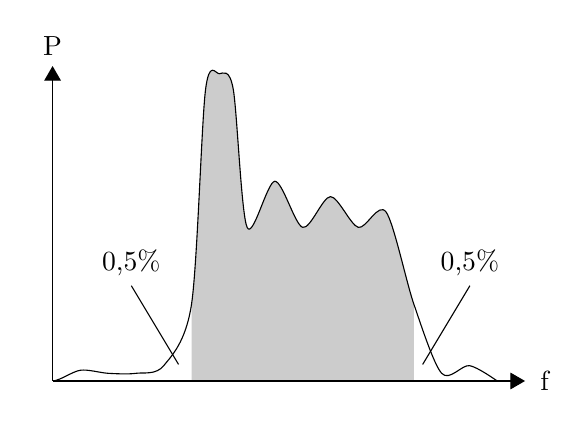
\begin{tikzpicture}
    \draw (0,4.25) node[]{P};
    \draw (6.25,0) node[]{f};

    %A:
    \draw (1.0,1.5) node[](A){0,5\%};
    \draw (5.3,1.5) node[](B){0,5\%};
    \draw (A.south) -- ++(+0.6,-1.0);
    \draw (B.south) -- ++(-0.6,-1.0);
    %B:
    %\draw (1,1.5) node[](A){5,0\%};
    %\draw (5.3,1.5) node[](B){5,0\%};
    %\draw (A.south) -- ++(+0.6,-1.0);
    %\draw (B.south) -- ++(-0.6,-1.0);
    %C:
    %\draw (3.5,3.0) node[](A){95\%};
    %\draw (A.south) -- ++(-0.6,-1.0);
    %D:
    %\draw (3.5,3.0) node[](A){98\%};
    %\draw (A.south) -- ++(-0.6,-1.0);

    \begin{axis}[%
        /pgf/number format/1000 sep={ },
        /pgf/number format/use comma,        
        axis lines=middle,
        axis line style={-triangle 60},
        width=6cm,
        height=4cm,
        scale only axis,
        every major tick/.append style={thick, black},
        grid=major,
        grid style={line width=.1pt, draw=gray!10},
        major grid style={line width=.2pt,draw=gray!50},
        xticklabel=\empty,
        yticklabel=\empty,
        xtick style={draw=none},
        ytick style={draw=none},
        xmin=3,
        xmax=20,
        ymin=0.0,
        ymax=20.5,
        xmajorgrids=false,
        ymajorgrids=false,
        tick label style={font=\footnotesize}
    ]
    \addplot[color=black,name path=B] coordinates{
        (0,0)
        (1,0)
        (2,0)
        (3,0)
        (4,0)
        (5,0)
        (6,0)
        (7,0)
        (8,0)
        (8.5,0)
        (9,0)
        (9.5,0)
        (10,0)
        (11,0)
        (12,0)
        (13,0)
        (14,0)
        (15,0)
        (16,0)
        (17,0)
        (18,0)
        (19,0)
    };
    \addplot[color=black,smooth,name path=A] coordinates{
        (0,0)
        (1,0.5)
        (2,0.5)
        (3,0)
        (4,0.7)
        (5,0.5)
        (6,0.5)
        (7,1)
        (8,5)
        (8.5,18.9)
        (9,20.0)
        (9.5,19)
        (10,10)
        (11,13)
        (12,10)
        (13,12)
        (14,10)
        (15,11)
        (16,5)
        (17,0.5)
        (18,1.0)
        (19,0)
    };
    \addplot[gray, fill opacity=0.4] fill between[of=A and B,soft clip={domain=8:16}];

\end{axis}
\end{tikzpicture}%
\end{document}

